\section{The evidence model}
\label{sec:evidence-model}

\subsection{The claim record}

The atomic unit of the whole PoC is the \code{ClaimRecord}
(\repo{residual/src/residual/claims.py}), a frozen \code{pydantic} model with fields
\code{assertion}, \code{question}, \code{layer}, \code{knowledge_type}, \code{tacitness},
\code{scope}, \code{evidence}, \code{generation}, \code{derivation}, \code{searches}, and
\code{certainty}. \evobs{} A claim needs at least one of \code{evidence}, \code{searches}, a
\code{derivation}, or a model \code{generation} to exist at all. An assertion must be non-empty and
whitespace-normalized. \code{certainty} may only be set on a claim whose label is one of the three
that can act as a criterion (\cref{tab:labels}). Claims live inside a \code{Ledger}
(\repo{residual/src/residual/ledger.py}), which also holds \code{Contradiction} and \code{Area}
records and a \code{purpose} field restricted to \code{reconstruction}, \code{gold}, or
\code{surrogate}. A \code{gold} ledger holds only criterion-labeled claims. A \code{surrogate}
ledger holds only simulation output. The three never share a ledger, so held-out gold cannot be
contaminated by reconstruction or synthetic material. \Cref{fig:evidence} shows how a claim ties
back to the text that produced it.

\begin{figure}[tbp]
  \centering
  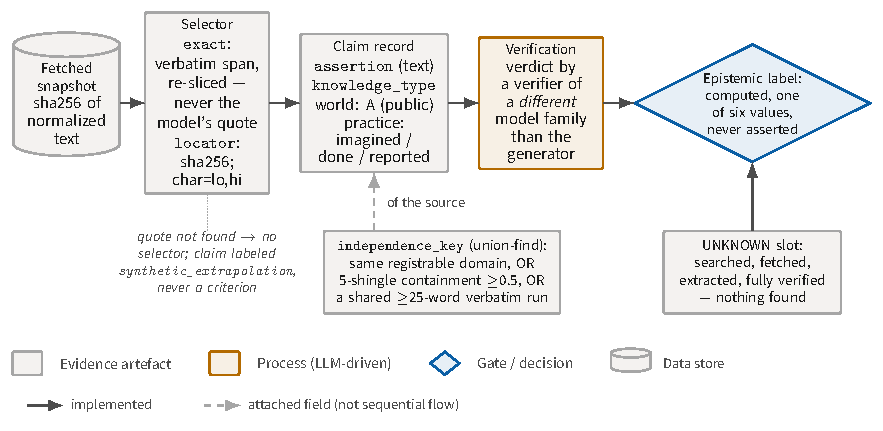
\includegraphics{figures/pdf/fig05_evidence.pdf}
  \caption[Provenance chain and label computation]{How a claim stays tied to its source: a
  fetched document is hashed once into a snapshot; a selector names an exact character span inside
  that hash; \code{ClaimRecord.label} is computed from the resulting evidence, never set by hand.}
  \label{fig:evidence}
\end{figure}

\subsection{Six epistemic labels, three of them criteria}

Every claim carries exactly one label, drawn from a closed enumeration
(\code{EpistemicLabel}, \repo{residual/src/residual/vocab.py}). \Cref{tab:labels} gives the exact
enum values and their plain-English meaning. \evobs{} Only three labels may ever act as a gate's
criterion (\code{CRITERION_LABELS}). A \code{Measurement} built by \code{gates.measure()} keeps
criterion labels apart from predictor labels. \code{evidential_gate} raises
\code{SyntheticRefused} on any \code{synthetic_extrapolation} input, and \code{GateRefusal} on
anything else outside \code{CRITERION_LABELS}, before the wrapped function runs at all. This is
the code form of the project's central rule: \textbf{synthetic output may be a predictor, never a
criterion}. A gap-map score, being derived from synthetic and inferred material, can rank
candidates for a human to look at; it can never decide a gate on its own.

\begin{table}[tbp]
  \centering
  \small
  \caption{The six epistemic labels (\code{residual.vocab.EpistemicLabel}), exact enum values.
  The first three are \code{CRITERION_LABELS}: the only labels an \code{evidential_gate} accepts.}
  \label{tab:labels}
  \begin{tabularx}{\linewidth}{@{}lXc@{}}
    \toprule
    Enum value & Plain-English meaning & May act as a criterion \\
    \midrule
    \code{observed_human_evidence} & Supported by a World C (human-record) source, or a
      human-record kind within World A & Yes \\
    \code{literature_supported} & Supported by a verified span in a public (World A) source & Yes \\
    \code{organisational_artefact_supported} & Supported by a verified span in an organization's
      own (World B) artifact & Yes \\
    \code{inferred} & No direct support, but derived from other claims via a \code{Derivation} & No \\
    \code{synthetic_extrapolation} & Produced or supported only by a model, with no verified
      human-authored span & No \\
    \code{unknown} & Searched for, fetched, and fully examined by another model family; nothing
      found & No \\
    \bottomrule
  \end{tabularx}
\end{table}

\subsection{The label as a computed property}

\code{ClaimRecord.label} is a Python \code{@property}, never a stored field: nothing in the code
base can set a claim's label directly. \evobs{} \repo{residual/src/residual/claims.py}
computes the label by a fixed rule, checked in this order. \emph{Supporting}
evidence means a SUPPORTS verdict after every exclusion reason --- self-verification, a
machine-voiced source, a software verifier, the wrong evidence world for the question --- returns
\code{None}:
\begin{enumerate}[noitemsep]
  \item simulated $\rightarrow$ \code{synthetic_extrapolation};
  \item supported by a World~C source, or a human-record-kind World~A source $\rightarrow$
    \code{observed_human_evidence};
  \item supported by a World~B source $\rightarrow$ \code{organisational_artefact_supported};
  \item supported by any other evidence $\rightarrow$ \code{literature_supported};
  \item an existing \code{Derivation} with no support $\rightarrow$ \code{inferred};
  \item a model \code{generation} with no support $\rightarrow$ \code{synthetic_extrapolation};
  \item otherwise $\rightarrow$ \code{unknown}.
\end{enumerate}
\code{Ledger.label} then
extends this for derived claims: an inference takes the \emph{weakest} of its premises' labels
(synthetic beats unknown beats inferred), so a chain of reasoning cannot bootstrap a strong label
from a weak one.

\subsection{Provenance chain}

Every fetched document is normalized exactly once (NFKC, quote/dash/bullet unification, whitespace
collapse) and hashed: \code{sha256:<text>}. \evobs{} A \code{Selector}'s \code{locator} names an
exact character span inside that hash, \code{sha256:<hash>;char=<start>,<end>}, and its
\code{exact} field is the literal slice of the normalized text -- never the model's own quotation.
A quote that cannot be located verbatim in the fetched text produces no \code{Evidence} at all. A
claim gains \code{Evidence} only through this re-slicing, which is why \code{verify_run.py} can
re-check every \emph{evidence item} in a run offline against its stored snapshot with no model
call. The chain is therefore: \textbf{snapshot hash} $\rightarrow$ \textbf{selector exact span,
re-sliced from the snapshot} $\rightarrow$ \textbf{claim}. Evidence from a quotable source kind is
required to carry an exact quote by a validator, not merely by convention.

\evobs{} This chain is independently checkable. \code{reconstruct.verify\_run} passes on all 909
evidence items across the three ledgers this report cites (PLC v1, GDPR v1, GDPR v2), re-slicing
every one against its stored snapshot with no model call. A separate, smaller sample was also
re-sliced by hand: 71 of 71 (\cref{app:claims}, row E25). Not every extraction reaches this chain.
When an extractor's proposed quote cannot be located, no \code{Evidence} is produced, and the claim
stays in the ledger with no supporting span. It is then labeled \code{synthetic\_extrapolation}:
418 of 1{,}169 claims across the three runs (49 PLC, 64 GDPR v1, 305 GDPR v2). For a slot that was
searched and fully verified with nothing found, the label is \code{unknown} instead: 34 more
(5, 14, 15). Together the two labels cover 452 of 1{,}169 claims (39\%) with no supporting span.
Such a claim is \textbf{not dropped}. Memorized model content can therefore enter the ledger, but
only under a label that cannot act as a gate's criterion (\cref{tab:labels}), so no lens or gate
reads it as a fact about the domain.

\subsection{Independence and contradictions}

Corroboration counts independent sources, not documents: \code{ClaimRecord.corroboration} is the
number of distinct \code{independence_key} values among a claim's supporting evidence. \evobs{}
Independence itself is computed by union-find over fetched documents
(\repo{reconstruct/src/reconstruct/evidence.py}, \code{independence_clusters}). Two documents
merge into one cluster when their registrable domain matches (a hand-listed set of
multi-organization domains, e.g.\ \code{arxiv.org}, is grouped by full host instead), or when
their 5-shingle containment is at least 0.5. A separate, span-level rule collapses syndicated
\emph{spans} of at least 25 verbatim words into one corroboration count without merging the
documents' clusters. This is a deliberate departure from an earlier whole-document rule that
over-merged unrelated documents (\cref{sec:n2}). Contradictions are a first-class \code{Ledger} record, not a
flattening step: when two claims from \emph{different} clusters, sharing an area, are cross-checked
and one verdict comes back REFUTES, that becomes a \code{Contradiction}.

\subsection{UNKNOWN is a searched-and-not-found result, never a blank}

A \code{ClaimRecord} with no evidence enters a reconstruction ledger under exactly one condition:
its (area, probe) slot was searched, fetched, extracted, and fully verified by another model
family, and nothing was found. \evobs{} Every weaker state -- \code{thin} (one supporting cluster,
not two), \code{unverified} (fetched but not fully verified), \code{unexamined} (nothing fetched) --
is tracked separately and never folded into \code{unknown}. This distinction matters because the
gap map's retrieval-gap category \code{RG-UNK} reads from exactly these \code{unknown}/\code{thin}/
\code{unverified} slots (plus ledger U-claims). A slot that was never searched is a retrieval
failure to fix, not an unstated fact about the domain.

\subsection{Evidence worlds and practice, as typed fields}

Three evidence worlds are a typed field on \code{Source}, not a narrative label:
\code{World.A = "public"}, \code{World.B = "organisational"}, \code{World.C = "human"}
(\repo{residual/src/residual/vocab.py}). \evobs{} A validator on \code{Source} requires a World~C
source to be a human-record kind, and requires exactly World~B sources to name their
\code{organisation}. A second typed field, \code{Practice}, distinguishes \code{imagined}
(prescribes work), \code{done} (records work), and \code{reported} (an account of work) -- the
Safety-II distinction between work-as-imagined and work-as-done. Both fields exist and are
enforced by the schema. \textbf{Only World A is populated in the PoC}: every N2 run to date
reconstructed from open-web text only, World~B has no ingestion adapter yet, and World~C has no
data at all.\footnote{Track A's instrument produces World~C-shaped records but is frozen outside
the NOW program (\cref{sec:scope}).}

\subsection{Residual accounting and the frozen schema, briefly}

\enquote{Residual accounting} names computing, per area, how much of a domain's claims carry each
epistemic label, and specifically how much of a target competence has no criterion-labeled support
at all. \evint{} \code{AreaFeatures} (per-area label, source-kind, tacitness, and contradiction
counts) and \code{ResidualAccount}/\code{EstimatedResidual} exist as types, and N2 computes the
features from real ledgers. But nothing yet computes an actual residual number against gold,
because no gold has been acquired. Decision 0006 hash-freezes the schema, the gap-map feature set,
and the label-deciding code together in \repo{residual/frozen/n1.json}. A \code{pytest}
architecture test fails if the live fingerprint diverges from the committed file, and changing any
of it needs a deliberate re-freeze and a commit explaining why. The exact fields, the three
SHA-256 hashes, and what each one covers are detailed in \cref{app:reproduce}.
